\documentclass[aspectratio=169]{beamer}
\setbeamertemplate{navigation symbols}{}
\usepackage{color,amsmath,comment, subfigure}
\usepackage{booktabs}
\usepackage{url}


%%%%%%%%%%%%%%%%%%%%%%%%%%
\title[]{Class 15: Complex contagion}
\author[]{Matthew J. Salganik}
\institute[]{Sociology 204: Social Networks\\Princeton University}
\date[]{
2/2 Experimental test of network structure on spreading
\vfill

\begin{flushleft}
\vspace{0.6in}

\includegraphics[width=0.1\textwidth]{figures/cc.png}
\end{flushleft}
}

\begin{document}
%%%%%%%%%%%%%%%%%%%%%%%%%%%
\frame{\titlepage}
%%%%%%%%%%%%%%%%%%%%%%%%%%%
\begin{frame}

\setcounter{subfigure}{0}
\begin{figure}
  \centering
     \subfigure{
     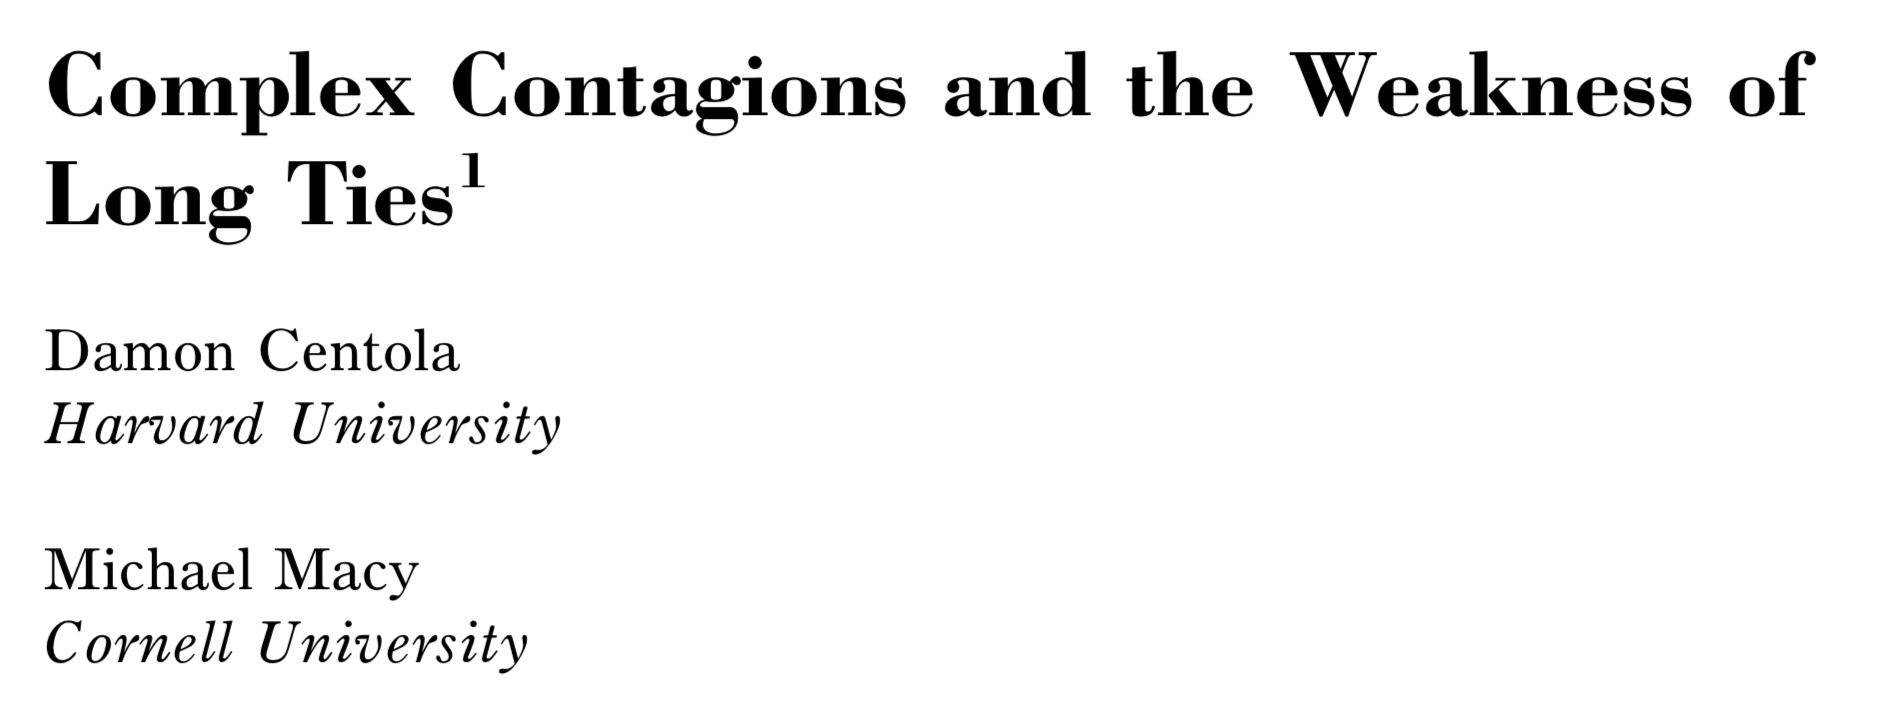
\includegraphics[width=0.45\textwidth]{figures/centola_complex_2007_title}}
  \hspace{0in}
    \subfigure{
    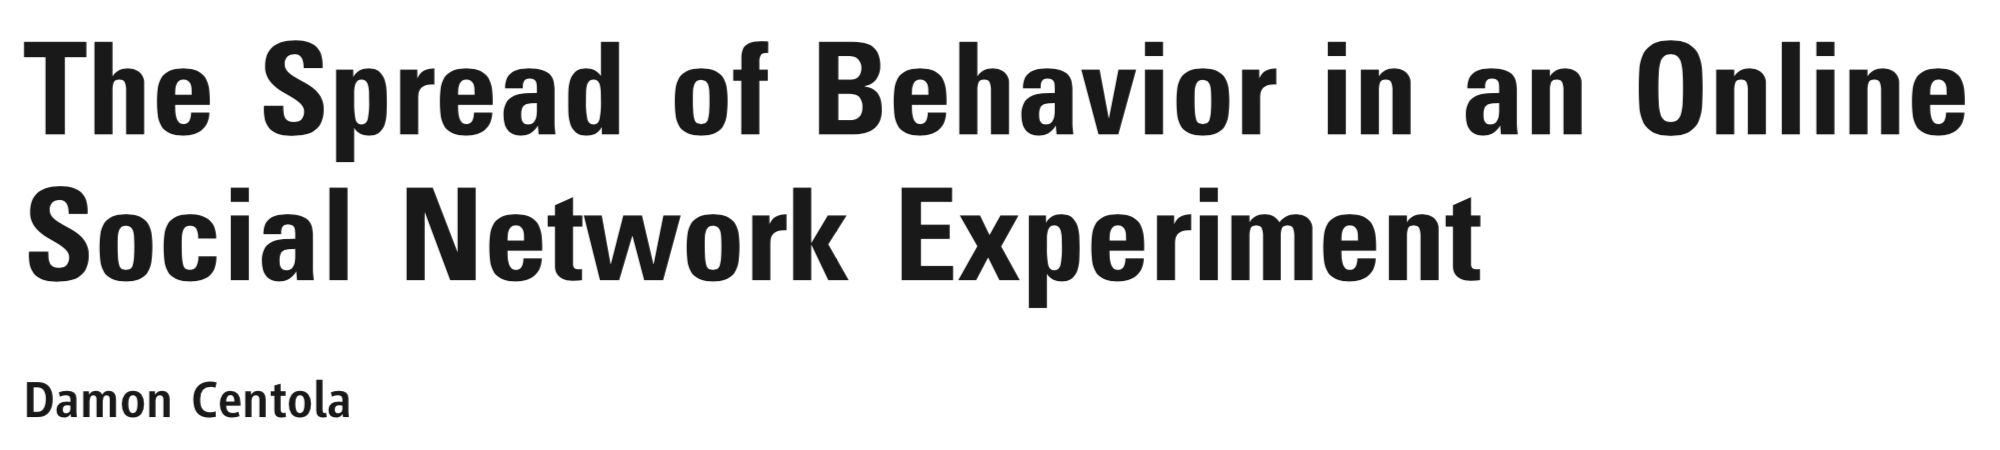
\includegraphics[width=0.45\textwidth]{figures/centola_spread_2010_title}}
\end{figure}


\end{frame}
%%%%%%%%%%%%%%%%%%%%%%%%%%
\begin{frame}

Two competing hypothesis:
\begin{itemize}
\item behavior will spread faster on highly clustered networks 
\item behavior will spread faster in networks with many ``long ties'' 
\end{itemize}

\begin{center}
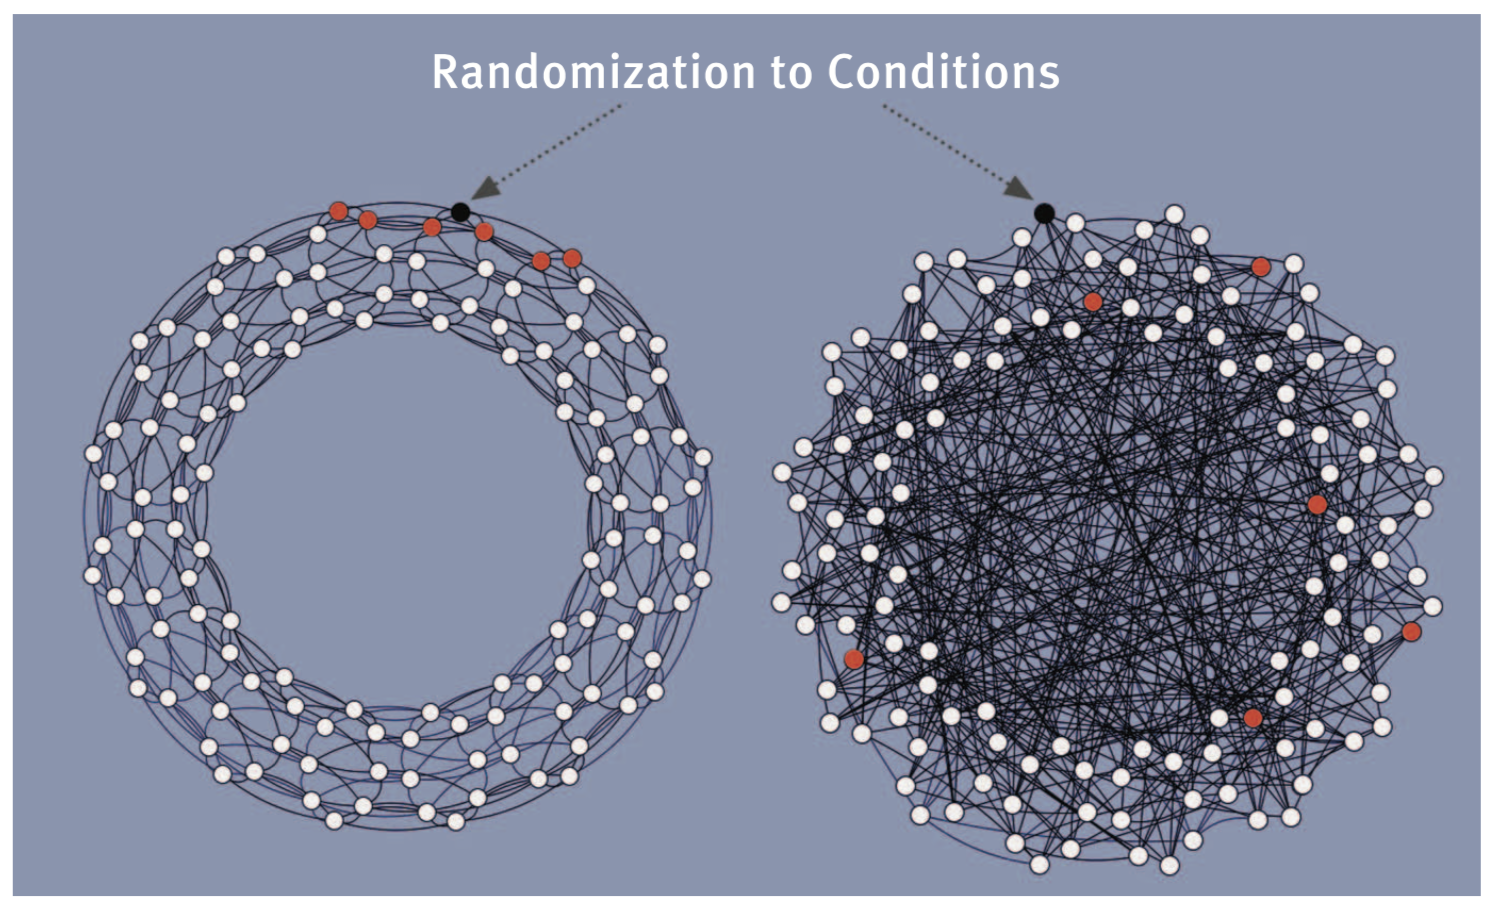
\includegraphics[width=0.5\textwidth]{figures/centola_spread_2010_fig1}
\end{center}


\vfill
Notice horse race design
\end{frame}
%%%%%%%%%%%%%%%%%%%%%%%%%%%
\begin{frame}

Let's listen to Damon tell us about the experimental set-up

\url{http://www.youtube.com/watch?v=o0fDcUJMzkI&t=47m52s}

\end{frame}
%%%%%%%%%%%%%%%%%%%%%%%%%
\begin{frame}

Let's listen to Damon tell us about the results

\url{http://www.youtube.com/watch?v=o0fDcUJMzkI&t=53m35s}

\end{frame}
%%%%%%%%%%%%%%%%%%%%%%%%%
\begin{frame}

\begin{center}
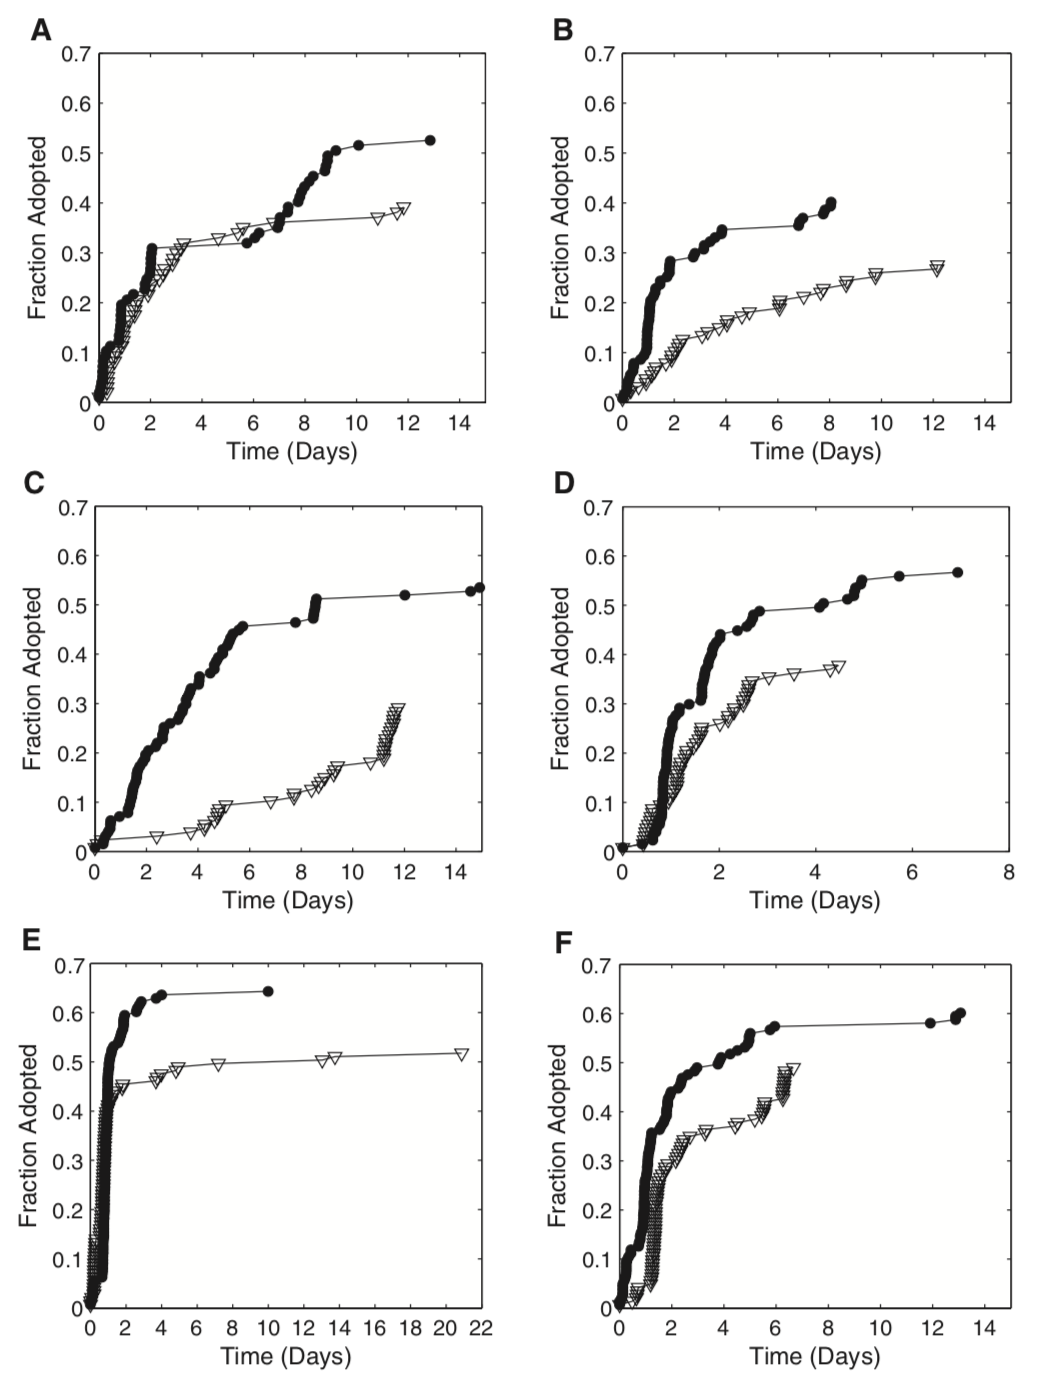
\includegraphics[height=0.8\textheight]{figures/centola_spread_2010_fig2}
\end{center}

\vfill
Behavior spreads further and faster in clustered network. This is because redundancy of emails helps with adoption.

\end{frame}
%%%%%%%%%%%%%%%%%%%%%%%%%%%
\begin{frame}

\begin{center}
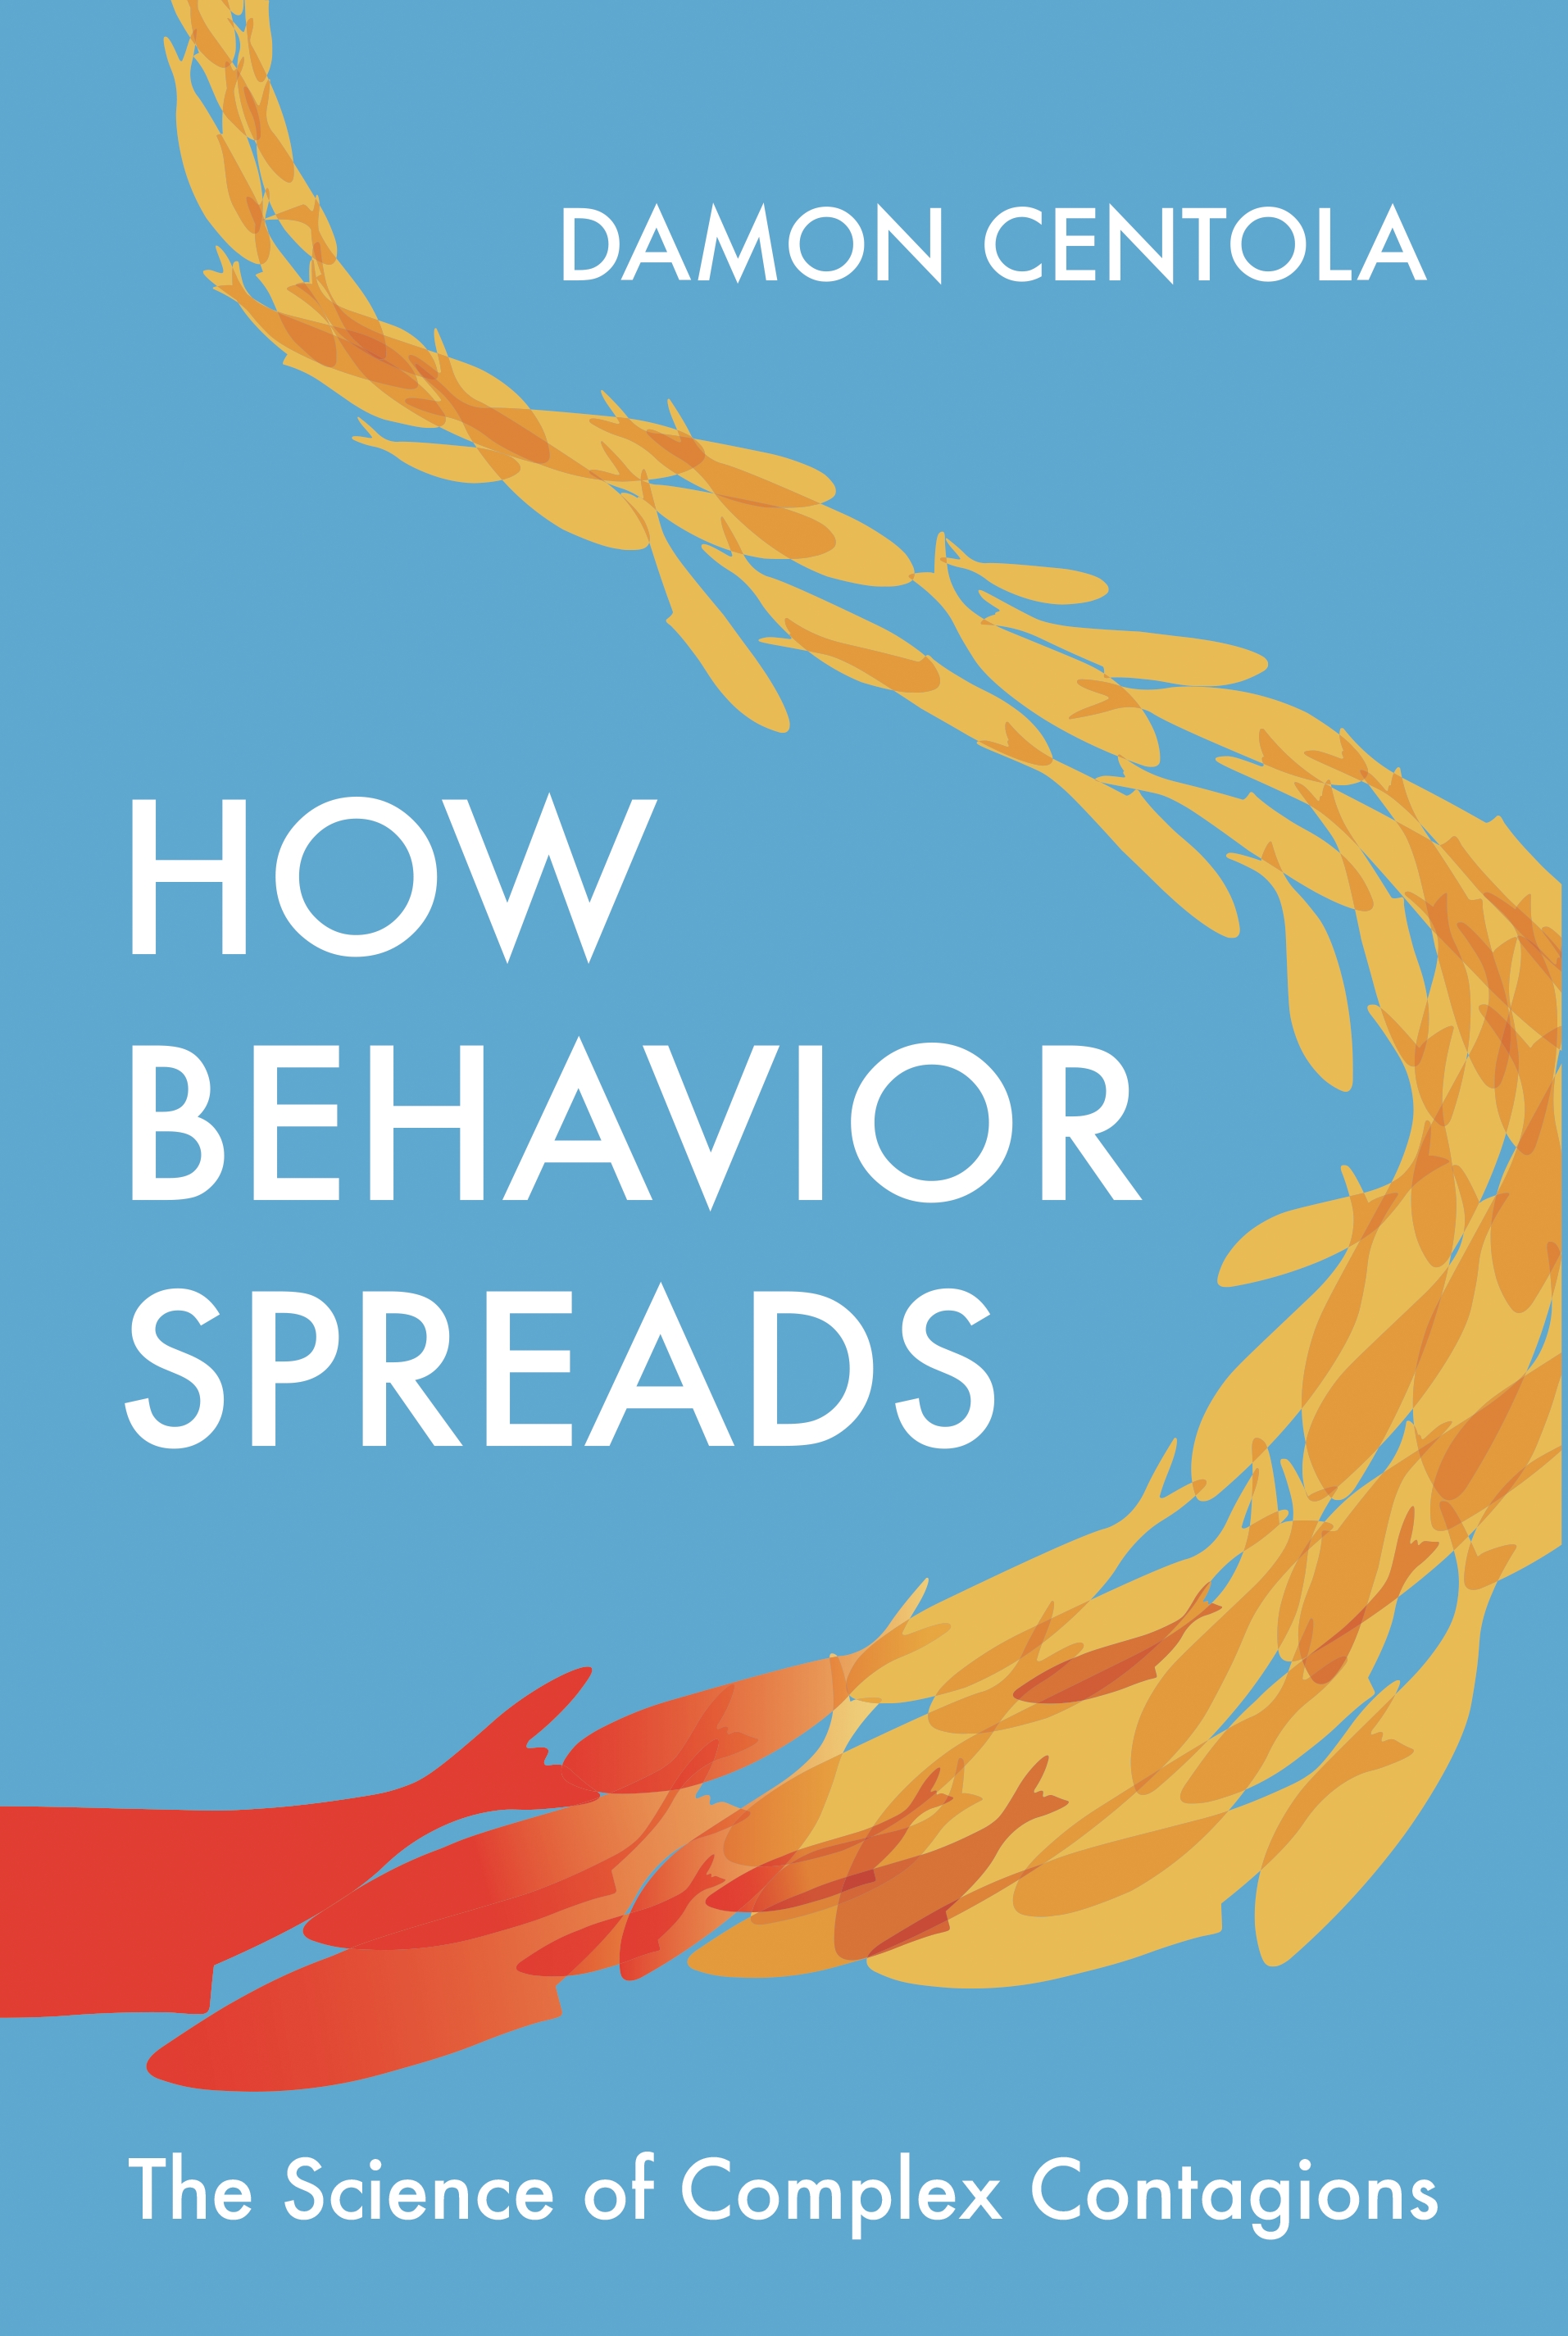
\includegraphics[height=0.8\textheight]{figures/centola_how_2018_cover}
\end{center}

\vfill
\url{https://www-jstor-org.ezproxy.princeton.edu/stable/j.ctvc7758p}

\end{frame}
%%%%%%%%%%%%%%%%%%%%%%%%%
\begin{frame}

Summary
\begin{itemize}
\item differentiate between simple and complex contagions (require 2 or more neighbors to be active) \pause
\item changes in network structure that promote simple contagion don't always promote complex contagion \pause
\item experiments showing that some behaviors spread more and faster in highly clustered networks rather than random networks \pause
\end{itemize}


Research design strategies
\begin{itemize}
\item replicate and extend \pause
\item horse race
\end{itemize}



\end{frame}
%%%%%%%%%%%%%%%%%%%%%%%%%
\begin{frame}

\begin{itemize}
\item Nickerson, D.W. (2008). Is voting contagious? Evidence from two field experiments. \textit{American Political Science Review}. 
\item Kramer, A.D.I. et al. (2014). Experimental evidence of massive-scale emotional contagion through social networks. \textit{Proceedings of the National Academy of Sciences}.
\end{itemize}

\end{frame}

\end{document}
